\section{PolyPasswordHasher: A New Technique for Password Verification}
\label{SEC:design}


The goal of PolyPasswordHasher is to make cracking individual passwords
infeasible.  It provides a way of preventing an attacker from validating a
password hash.  At its core, PolyPasswordHasher aims to protect password hashes
by combining a share (derived using a threshold cryptosystem) with a salted
password hash and then storing this combined value in the password database.
Neither the share nor the password hash is stored on disk and, as we discuss in
more detail below, an attacker cannot recover either piece with only the
password database.  Cracking a password that is stored by PolyPasswordHasher
requires that the attacker know a threshold of passwords; this effectively
makes the passwords in a database interdependent.  Our goal is to ensure that
so long as an attacker does not know a threshold of passwords, no password in a
database can be cracked.

To make passwords interrelate, \PPH functions differently from a salted hash.  A
typical salted hash database stores a Username, Salt, and a Salted Hash.  A \PPH
database, rather than storing a salted hash, stores the secure hash XORed with
the share (\sxh).  The resulting \PPH database also holds an extra field called the
share number.  This field indicates which share was XORed with which salted
hash.   

\begin{figure}
    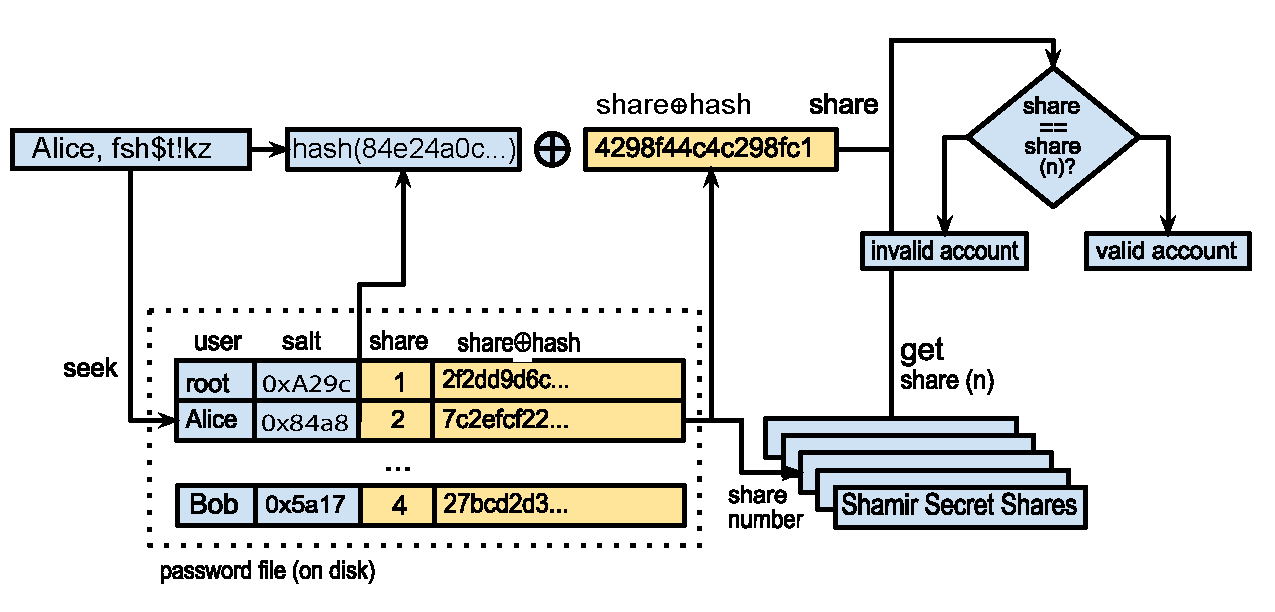
\includegraphics[width=1\linewidth]{./images/Verify_account.pdf}
    \caption{Account verification. }
    \label{FIGURE:account-verification}
\end{figure}


When prompted to validate a password, the server XORs the salted hash with the
stored data and determines whether the result is a valid share of the threshold
%cryptosystem.  For example, in Figure~\ref{FIGURE:basic-pph-algorithm}, Bob
cryptosystem.  For example, in Figure~\ref{FIGURE:account-verification}, Alice
has provided her password (`fsh\$t!kz') and the username `Alice'.  
The server and computes the salted hash of her password (`4298f44d...') and
reconstructs Alice's share (`3e773b6f...') using her share number
(2).  The server XORs the share and Alice's salted password hash together
and compares them to the value stored in the \sxh field in the password
database (`7cefcf22...').  If they match, then the password
provided was correct.

Account creation involves creating a share and XORing it with
the salted hash of the password before storing it on disk 
For example, in Figure~\ref{FIGURE:basic-pph-algorithm}, Bob registers an
account with his password (`Tr4mP0l1ne') and username (`Bob').  The 
server computes a salt (`0x5a17') and the salted hash of Bob's
password (`4153f0aa...').  The server knows the secret and knows Bob's
share number, 4. It computes Bob's share (`66ef2279...') and this value is XORed
with Bob's password’s salted hash; that value is compared to the value
stored in the database (`27bcd2d3...'). If these match, then the password
provided was correct.
%cryptosystem.  For example, in Figure~\ref{FIGURE:basic-pph-algorithm}, Bob

\begin{figure}
    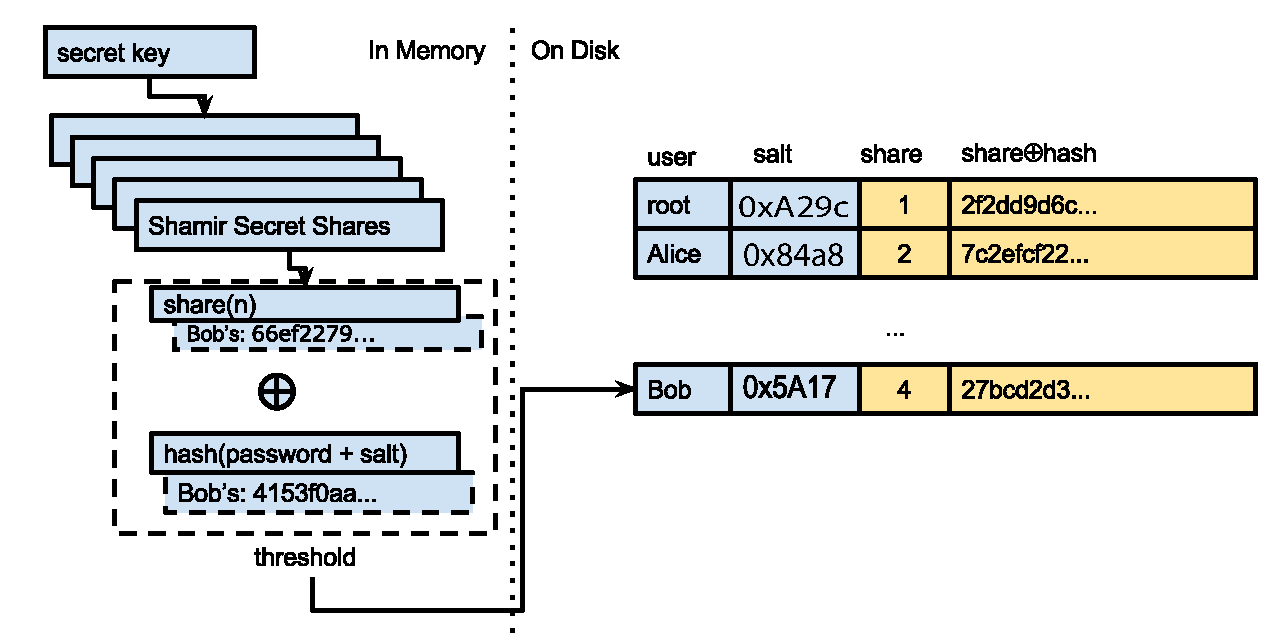
\includegraphics[width=1\linewidth]{./images/basic-pph-algorithm.pdf}
    \caption{The basic PolyPasswordHasher algorithm showing how an entry is created}
    \label{FIGURE:basic-pph-algorithm}
\end{figure}

In PolyPasswordHasher, each share protects a salted hash and each salted hash
protects a share, unless a threshold of shares is known (as is shown in
Figure~\ref{FIGURE:pph-interdependency-2}).  Suppose that an attacker has
obtained the password database and knows some set of account passwords (x,y,z).
For each known password, (illustrated in Figure~\ref{FIGURE:pph-interdependency-new}) 
the hacker can compute the salted hash and XOR this with the database entry to 
obtain the corresponding share.  If the attacker does not have a threshold of shares, 
the attacker cannot generate a share for another account (e.g., `share a').  As a 
result, the attacker cannot access share a's password's salted hash and cannot crack 
a's password.  Or, suppose that a server has a threshold of correct passwords.  
The server now has enough information to validate a threshold of shares and can use those to
recover the secret. The server could then reconstruct any share and thus,
recover the salted hash for any account's password -- an important step in
validating passwords.  Because shares protect passwords, an attacker who does
not have an adequate number of correct passwords (and thus shares) cannot
feasibly crack passwords individually. 

\begin{figure}
    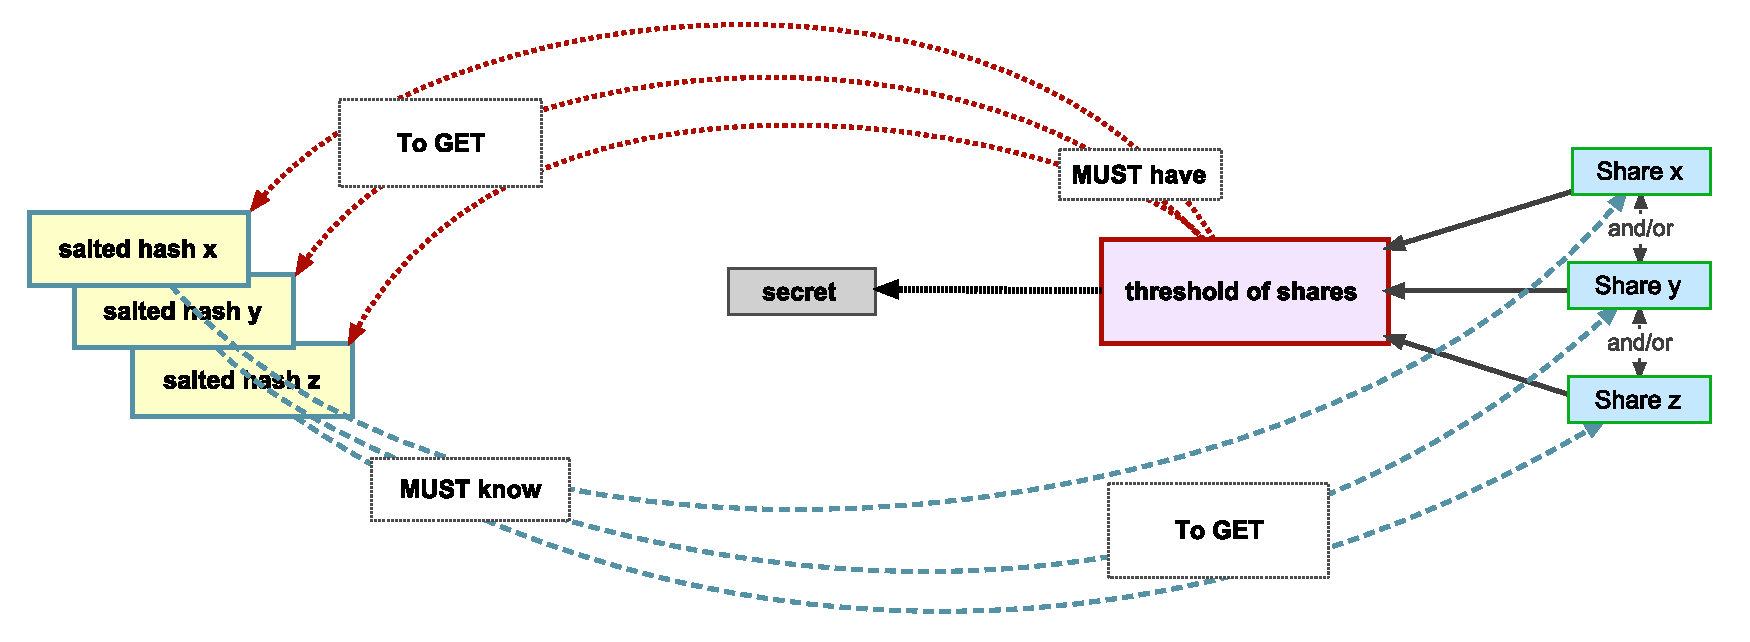
\includegraphics[width=1\linewidth]{./images/pph-interdependency-2.pdf}
    \caption{An attacker: (1) Cannot obtain salted hashes (needed to crack
    passwords) without a threshold  of shares AND (2) Cannot obtain a share without
    knowing the salted hash (password) for a \thresholdaccount.}
    \label{FIGURE:pph-interdependency-2}
\end{figure}

\begin{figure*}
    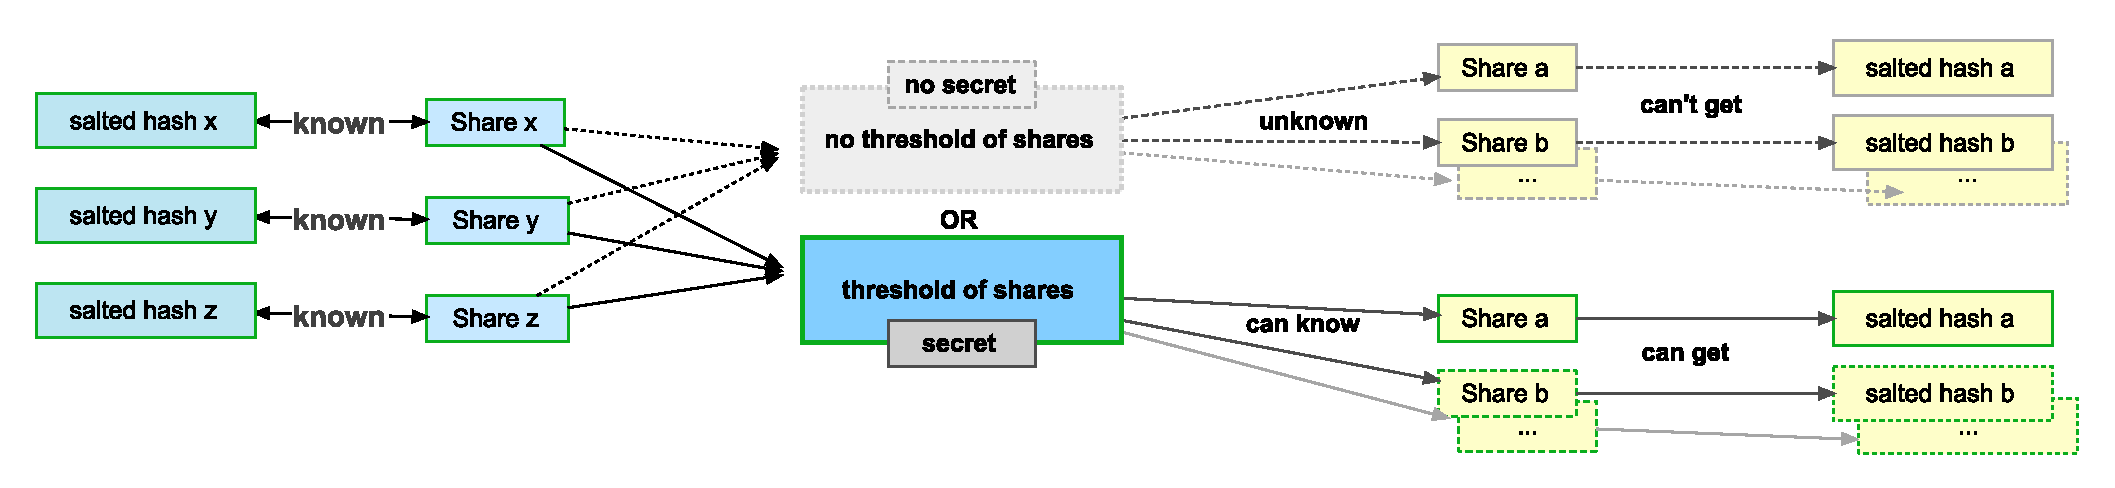
\includegraphics[width=1\linewidth]{./images/pph-interdependency-new.pdf}
    \caption{If an attacker knows some number of shares he can get the
    corresponding salted hashes; if he knows the salted hashes, he can get the
    corresponding shares; and, if he has a threshold of these, he can get the
    secret.}
    \label{FIGURE:pph-interdependency-new}
\end{figure*}
    
The basic scheme, as outlined so far, covers PolyPasswordHasher’s core 
functions.  In the remaining subsections we address how \PPH checks passwords 
without having a threshold of correct passwords (such as after a restart) and 
how it ensures that all
accounts, even those that could be created by an attacker, are protected.  To
more fully describe the full \PPH algorithm, we begin, in
Section~\ref{SUBSEC:normal-operation}, with how PolyPasswordHasher functions in
situations where the server has already validated a threshold of correct
passwords and how, after reaching this threshold, the server proceeds to login
normal users, in a phase we call normal operation.  Following this,
Section~\ref{SUBSEC:bootstrapping} discusses how \PPH performs differently when
a threshold of correct passwords have not yet been provided and needs to
acquire that threshold (e.g. after a reboot).
Section~\ref{SUBSEC:bootstrap-transitioning} discusses how the system
transitions between bootstrapping and normal operation and in
Section~\ref{SUBSEC:handling-rare-events}, we describe how unlikely situations,
such as the loss of a large number of account passwords, are handled.

\subsection{Normal operation of PolyPasswordHasher}
\label{SUBSEC:normal-operation}

Given that a server with a threshold of shares can effectively recover any
salted hash, if every account protected a share, every password would play an
important role in protecting the security of the database.  However, not all
accounts should necessarily be trusted to protect shares.  For example, a forum
may allow any user to register an account and any party, including an attacker,
to register any number of user accounts.  If these accounts each protected a
share, an attacker could easily crack the password database.

PolyPasswordHasher enables one group of passwords, which we call protector
accounts, to protect the remaining passwords in the password database; these we
call \thresholdlessaccounts.  Bob's account (who we started following in the
previous example) is an example of a \thresholdaccount
(Figure~\ref{FIGURE:protected-protector}).  An administrator will define a
threshold value of \thresholdaccounts so that if an attacker does not know a
threshold of protector passwords, Bob's salted hash cannot be recovered.  Bob's
password hash protects his share and in turn, Bob's share helps to protect the
other shares (such as shares 1,2), which in turn protect their corresponding
password hashes (for root and Alice). These shares serves to protect the full
password database, including \thresholdlessaccounts (Trudy and Luke). 

\begin{figure}
    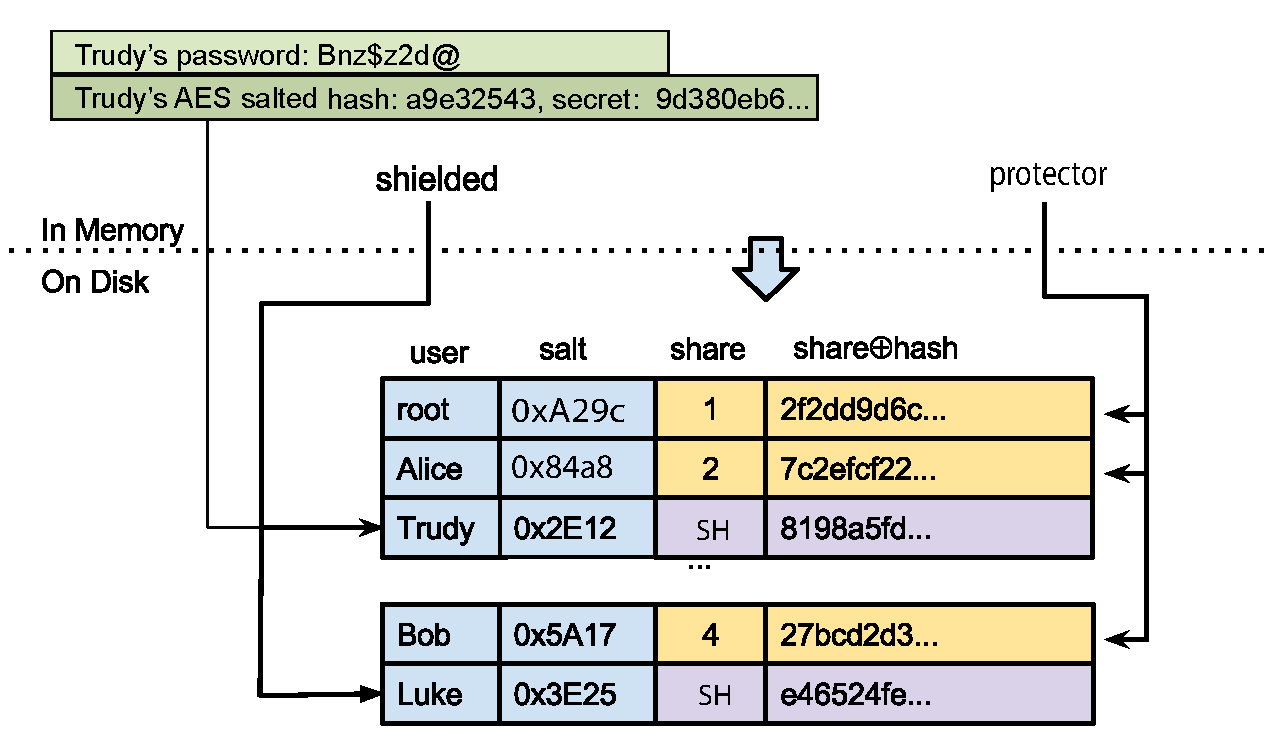
\includegraphics[width=1\linewidth]{./images/pph-store.pdf}
    \caption{A PolyPasswordHasher store with protector and \thresholdlessaccounts. \Thresholdlessaccounts are displayed with a share number of SH. }
    \label{FIGURE:protected-protector}
\end{figure}

Since a \thresholdlessaccount  does not protect a share, it is not XORed with one.
Nonetheless, these accounts are still protected by shares, or more precisely,
the secret.  \PPH uses the secret as an encryption key and with it, encrypts the
password's salted hash.  For these accounts, the resulting value (but not the
secret or salted hash) is stored in the password database.  For example, in
Figure~\ref{FIGURE:protected-protector}, Trudy's password hash (a9e32543...) is
encrypted using the secret (9d380eb6...); the result (8198a5fd...) is stored in the
database.  There are two important points to note.  First, if an attacker knows
another \thresholdlessaccount's password (e.g., Luke's), this does not
substantially help with cracking Trudy's password.  The attacker would need to
break the symmetric encryption algorithm.  Also, knowing Luke's
password would not substantially help the attacker crack the secret or other
shares in the password.  Once again, the attacker would need to break the
symmetric encryption algorithm.  Thus, \thresholdlessaccounts cannot be
effectively cracked unless an attacker knows a threshold of \thresholdaccount 
passwords.

\subsubsection{PolyPasswordHasher's algorithm}
\label{SUBSUBSEC:pph-algorithm}

Algorithm~\ref{ALG:acc-creation} details the processes of creating a user 
accounts.  The relevant operations for normal operation (lines 2-13)
are discussed in this section.  Bootstrapping operations (lines 14-23) are
deferred to the next section.

\begin{algorithm}
\footnotesize
\begin{algorithmic}[1]\Function{createAccount}{username, salt, saltedPasswordHash, isProtectorAccount}
    \vspace{.1cm}
    \State \codecomment{\footnotesize// check whether we are under normal operation}

    \If{normalOperation} \codecomment{\footnotesize// Section \ref{SEC:design} and 
    \ref{SUBSEC:normal-operation}}

        \If{isProtectorAccount} 

            \State \codecomment{\footnotesize// Obtain a share from the share cryptosystem}
            \State shareNumber, share = SecretShares.getShare()
            
            \State \codecomment{\footnotesize// Combine the share with the hash}
            \State passwordEntry = share $\oplus$ saltedHash
            \State shareID = shareNumber

        \vspace{.11cm}
        \Else~\codecomment{\footnotesize// Shielded Account 
        (Section~\ref{SUBSEC:normal-operation})}
            \State Key = SecretShares.getSecret() 
            \State passwordEntry = AES.encrypt(saltedPasswordHash, Key)
            \State shareID = \THRESHOLDLESS
        \EndIf

    \vspace{.1cm}
    \Else~\codecomment{\footnotesize// Bootstrapping (Section~\ref{SUBSEC:bootstrapping})}

        \If{isProtectorAccount}
            \State raise AccountCreationError
        \Else
            \State shareID = BOOTSTRAP
        \EndIf 
        \State passwordEntry = saltedPasswordHash
    \EndIf

    \State \codecomment{\footnotesize// Isolated Validation (Section~\ref{SUBSEC:bootstrapping})}
    \State isolatedCheckBits = saltedPasswordHash.getSuffix(IC\_BITS)
    \State passwordEntry += isolatedCheckBits 

    \State store (username, salt, shareID, passwordEntry)
    \EndFunction

\end{algorithmic}
\caption{\small Account creation pseudocode.
\label{ALG:acc-creation}}
\end{algorithm}

{\bf Creating Accounts}.  Adding an account works as is shown in
Algorithm~\ref{ALG:acc-creation}.  As the algorithm describes, the username,
salt, the password’s salted hash, and a boolean are used to indicate whether or
not the account should be a \thresholdaccount. If the account is a
\thresholdaccount, an unused share is found (line 6) and the salted hash is
XORed with it (line 8) before the share number and resulting value are stored
(line 23).  

Since a \thresholdlessaccount does not protect a share, those accounts are
instead encrypted with the secret (lines 11-12).  The share field is set to a
special value that indicates a \thresholdlessaccount (line 13).  As before,
this information is then stored in the database (line 23).
 
It is important to prevent users, particularly \thresholdaccounts, from using bad
passwords.  Similar to many deployed systems, PolyPasswordHasher employs simple
techniques to weed out extremely bad passwords.  When creating an account,
users input a password they want to use, but \PPH checks this password to ensure
that it is not too weak (e.g., ``letmein'' or ``password'').  This is done by
checking the requested password against a list of commonly used passwords (the
64K most popular). The proposed password will be rejected if it is on
that list.  PolyPasswordHasher also enforces constraints on the password length
and composition (number of lowercase and uppercase letters, numbers, and
symbols).  The purpose is not to ensure that passwords are immensely strong,
but to prevent the use of \thresholdaccount  passwords that are trivial to
guess.  These constraints are already common in many systems, such as those
that aim to prevent passwords from being cracked by brute force over the
network.  


{\bf Process for Verifying Passwords}. Assuming that the server holds the
right number of valid passwords (and thus shares), it will be able to recover
the remaining shares, as shown in Algorithm~\ref{ALG:acc-verification}.
To verify a \thresholdaccount  (lines 4-5), the server first computes the salted
hash of the user’s password and XORs it with the passwordEntry. If the
passwordEntry XORed with the salted hash is the share, then the password is
correct.  

For a \thresholdlessaccount, password verification differs because the salted hash
is encrypted instead of being XORed with a share.  Lines 8-10 of
Algorithm~\ref{ALG:acc-verification} describe how to compare the provided password
hash.  The password hash is encrypted with the secret and, if the encrypted
value matches the \sxh field, the correct password was provided.  




\begin{algorithm}
\footnotesize
\begin{algorithmic}[1]\Function{verifyAccount}{username, saltedPasswordHash, shareID, passwordEntry}

    \If{normalOperation}
        \If{isProtector(shareID)}\codecomment{\footnotesize // Section~\ref{SEC:design}}
            \State share = passwordHash $\oplus$ passwordEntry 
            \State return SecretShares.computeShare(shareID) == share
        \Else \codecomment{\footnotesize// \thresholdlessaccount , 
    Section~\ref{SUBSEC:normal-operation}}

            \State \codecomment{\footnotesize// Encrypt the obtained hash and compare}
            \State Key = SecretShares.getSecret()
            \State encryptedHash = AES.encrypt(passwordHash, Key)
            \State return passwordEntry == encryptedHash

        \EndIf
        \vspace{.1cm}

    \Else \codecomment{\footnotesize// Bootstrapping, Section~\ref{SUBSEC:bootstrapping}}

        \State \codecomment{\footnotesize// verify account created during bootstrap}
        \If{shareID == BOOTSTRAP}
            \State return passwordHash == passwordEntry
        \EndIf 

        \If{not passwordHash.endsWith(isolatedCheckBits)}
            \State return False
        \EndIf 
        \If{isProtector(shareID)}
            \State share = passwordHash $\oplus$ passwordEntry
            \State SecretShares.cacheShare(share)
        \EndIf
        \State return True

    \EndIf

    \EndFunction
\end{algorithmic}
\caption{\small Account verification pseudocode.\label{ALG:acc-verification}}
\end{algorithm}

{\bf Changing a user's password / password recovery} Changing a password
is a similar process to that used in a salted hash system, for both \thresholdaccounts
and \thresholdlessaccounts. Similar to existing systems, the procedure for
changing a password may require validating the existing password before
allowing a replacement to be generated. Changing the password involves creating
a new entry with the same username and share number. (This is nearly identical
to account creation.)  A new salt is generated and hashed along with the new
password.  Since the hash has changed, the fourth field will also change. Once
the new password entry is computed, it replaces the original stored data.  The
user may then log in normally with their new account.

\subsection{Bootstrapping After a Reboot}
\label{SUBSEC:bootstrapping}

When a system restarts, \PPH cannot validate or create accounts as it normally
would, because a threshold of valid accounts has not been reached. Because \PPH
stores shares in memory, not on disk, these are lost during reboot.  This means
that a server does not know the secret and cannot compute arbitrary shares.  As
a result, when bootstrapping, neither \thresholdaccount nor \thresholdlessaccounts 
may be verified or created using the methods described above; account creation and verification
procedures are different when the system is bootstrapping.  

%\begin{figure}
%    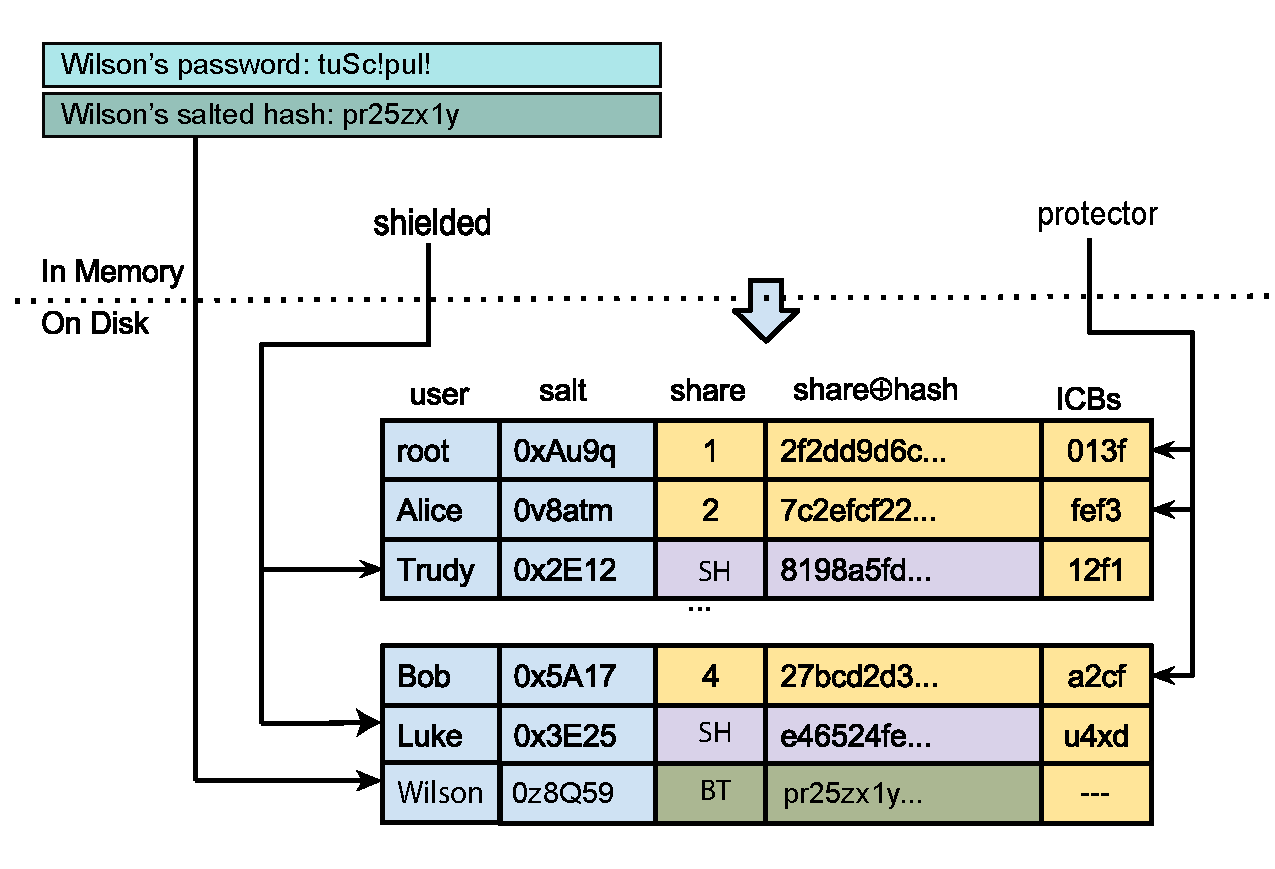
\includegraphics[width=1\linewidth]{./images/bootstrap}
%    \caption{Bootstrapping is similar to verifying an account except that we
%    use the obtained shares to restore the secret and interpolate the rest of the
%    shares.}
%    \label{FIGURE:bootstrap}
%\end{figure}

\subsubsection{Bootstrap account creation}
\label{SUBSUBSEC:bootstrap-account}

New accounts may also be created during bootstrapping. To do this, the new
account is added to the database along with the salted hash.  While the system
is bootstrapping, the new account is available to use.  In the interim, these
passwords will be created (line 19 of Algorithm~\ref{ALG:acc-creation}) and
validated (lines 18-19 of Algorithm~\ref{ALG:acc-verification}) in the same
manner as passwords stored in a system that uses salted hashes.

Although it would be easy to support \thresholdaccount creation during
bootstrap, PolyPasswordHasher does not do so (line 16 of
Algorithm~\ref{ALG:acc-creation}).  The reason is that an attacker who can
read the password database would also be able to read the salted password hash.
If the attacker can later read the password database during normal operation,
the attacker could use that salted password hash to recover the share. 

\subsubsection{Isolated Validation}
\label{SUBSUBSEC:isolated-validation}

When started, a \PPH system does not have enough protector passwords (and thus,
shares) to recover the secret.  At this point it is not possible to validate
accounts following the same process as \PPH's normal operation
(\ref{SUBSEC:normal-operation}).  Here we describe how \partialverification  can
be used to check logins even without the secret.  \Partialverification is a
process that leaks a configurable number of bits of the salted hash by using a
slow hash algorithm.  It implements a mechanism wherein it is possible, but
extremely unlikely, that an attacker could access an account using an incorrect
password.  In the next section we discuss the \partialverification mechanism,
but defer discussion of its algorithm until
Section~\ref{SUBSEC:security-properties}.

As it bootstraps, \PPH collects shares from protector logins. The number of
logins required to recover the secret will have been configured by the system
administrator, with the threshold normally set to a low number (e.g., three). 
Once the threshold has been reached, \PPH will finish bootstrapping
(Section~\ref{SUBSEC:bootstrapping}). Meanwhile, before this threshold is
reached, \partialverification makes use of an isolated-check bits field to authenticate
user passwords. 

In this scheme, illustrated in the upper right corner of
Figure~\ref{FIGURE:isolated-verification}, the password database contains
isolated-check bits.  These bits are used to verify logins before a threshold
is reached and the same process is used for both protector and shielded
accounts.  The user's password is hashed using the \partialverification hash
function.  This function returns a small number of bits of the hash (such as 24
bits of a SHA256 hash) and typically involves many iterations of a secure hash
function.  If the isolated-check bits field of the password database match the
\partialverification  hash function’s output (line 12 of
Algorithm~\ref{ALG:acc-verification}), the user is allowed to log in.

\begin{figure}
    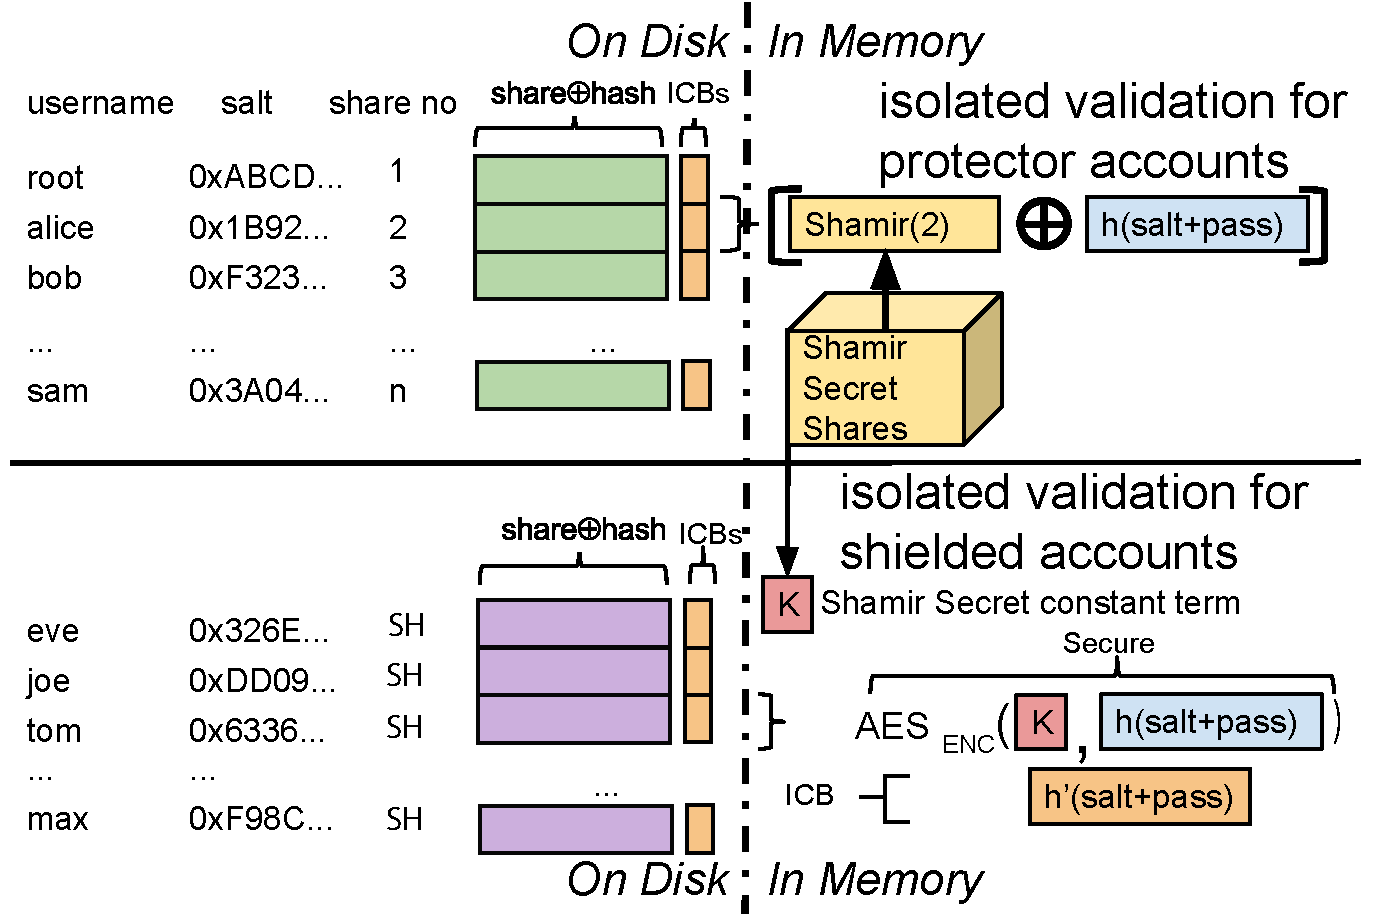
\includegraphics[width=1\linewidth]{./images/pph-with-partial-bytes.pdf}
    \caption{This figure shows validation using \partialverification. The
    isolated-check bits are stored on disk. This allows verification of accounts
    before a threshold of correct passwords is provided.  } 
    \label{FIGURE:isolated-verification}
\end{figure}

\begin{figure}
    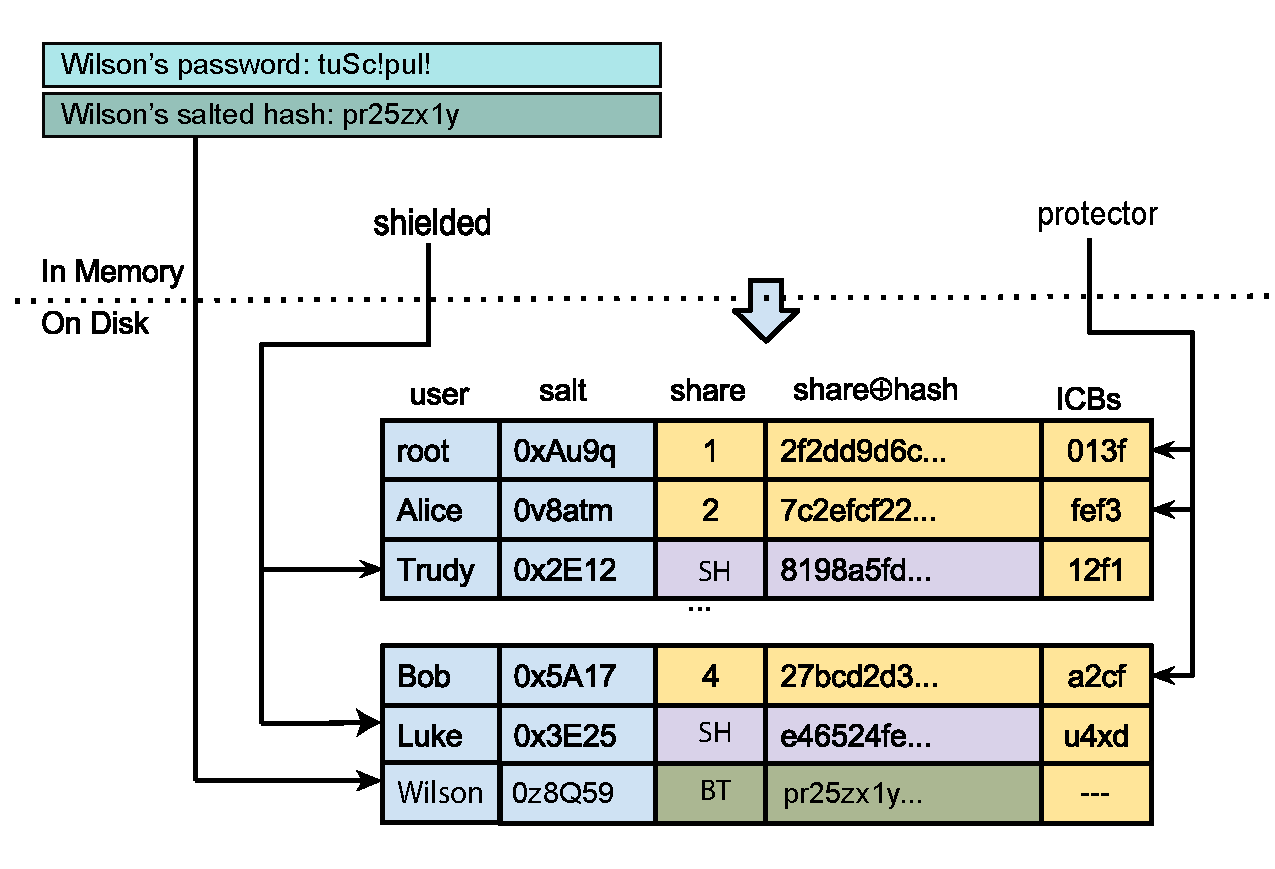
\includegraphics[width=1\linewidth]{./images/bootstrap.pdf}
    \caption{Wilson's account was created during bootstrap, so a regular
    salted hash is stored instead.} 
        \label{FIGURE:bootstrap-verification}
\end{figure}

For example, Figure~\ref{FIGURE:bootstrap-verification} illustrates 
verification while the system is bootstrapping.  Bootstrap accounts, such
as Wilson's account are validated in an identical way to a salted hash
system.  Wilson's password is salted and hashed and this is compared
with the value stored in the database.  If it matches, Wilson is logged in.

\Thresholdaccounts and \thresholdlessaccounts, like those of Trudy or Alice may
also log in while the system is bootstrapping
(Figure~\ref{FIGURE:bootstrap-verification}) using \partialverification.  The
\partialverification hash function is computed over the provided password and
the \partialbytes field is checked.  If these values match, the user is allowed
to log in. Bootstrap accounts, such as Wilson's account are validated in an
identical way to a salted hash system.  Wilson's password is salted and hashed
and this is compared with the value stored in the database.  If it matches,
Wilson is logged in.

\Partialverification represents a tradeoff for administrators.  Using 
\partialverification makes the system available immediately after a reboot.  
However, when using a small number of \partialbytes, there is the potential
for an incorrect authentication during the bootstrapping phase.  Alternatively
a large number of \partialbytes impacts the confidentiality of the password
database in the event of a theft, by making the passwords easier to crack.
Thus in some scenarios different settings are appropriate, possibly
even for \thresholdaccounts and \thresholdlessaccounts in the same database.
We explore this tradeoff more in Section~\ref{SUBSEC:security-properties}

\subsection{Transitioning From Bootstraping to Normal Operation}
\label{SUBSEC:bootstrap-transitioning}

As the system bootstraps, the server batches shares from \thresholdaccounts
(line 14 of Algorithm~\ref{ALG:acc-verification}).   After the system has a
threshold of shares, it is possible to recover the secret. The server performs
Lagrange interpolation, which allows the server to not only recover the secret
but also, to generate arbitrary shares (both are needed to check \thresholdlessaccounts).  

Recall that accounts created during the bootstrap phase contain BOOTSTRAP for
their share number and have a salted hash stored in the database.  When the
system recovers the secret and transitions to normal operation, these accounts
will have their password hashes encrypted with the secret and their share
number field set to \THRESHOLDLESS.  This transforms these accounts to the same
state as \thresholdlessaccounts that are created in normal operation.

Also, all account logins that were processed during bootstrapping are now
checked to be certain that the correct passwords were provided.  This step is
needed because it is possible that an attacker could find a password that is
invalid and yet, matches the \partialbytes.  (We examine the feasibility and
computational cost of this in Section~\ref{SEC:evaluation})  The salted
password hash for \thresholdlessaccount logins are cached in memory and the
passwords are verified once a threshold is reached.

For a \thresholdaccount , if a provided password hash matches the \partialbytes,
but the password is not correct, the recovered share is not invalid.  The
incorrect share will be detected when a threshold of shares are obtained
because the integrity check on the secret will fail.  If this integrity check
fails, the administrator is notified.  The system can still enter normal
operation once a threshold of valid shares are obtained.  

\subsection{Handling Rare Events}
\label{SUBSEC:handling-rare-events}

At an administrator's behest, accounts may be switched between shielded
and protector without user intervention. To do this, the server must be in
normal operation.  The server can then recover the salted secure hash. This
salted secure hash can then be re-encoded (using a share for an account that
becomes a \thresholdaccount; or encrypted, for an account that becomes
shielded) and the new entry can be stored. This transitions the account
from a protector to shielded (or vice versa).

{\bf Recovering data if all \thresholdaccounts are lost}.  If not enough
known threshold users can be verified, the salted hashes are lost forever and
accounts cannot be validated using the technique we described in
Section~\ref{SUBSUBSEC:isolated-validation}.  However, this does not mean that
the system is unusable because \partialverification allows users to log in.
Furthermore, mechanisms like root password recovery that are done through the console
will still work, and will allow any data on the system to be accessed.

{\bf Trusting a \thresholdaccount with multiple shares}.  A single
account may optionally provide access to multiple shares. 
To do this, a single user can have multiple rows in the table.  Each 
row will have a different \sxh entry and thus protect a different share.
Each entry must also have a different salt to ensure that a different
hash value is XORed with each share.  When the user provides their password,
the value can be used to recover the share in each row by XORing the salted
password hash with each share.

{\bf Detecting an \partialbytes match of an incorrect password}.  If the
system is in normal operation, it will detect that the password does not match.
However, PolyPasswordHasher will always check the \partialbytes for an entered
password (for clarity, not depicted in Algorithm~\ref{ALG:acc-verification}).
If the password is incorrect, but the \partialbytes match, this indicates that
an attacker has almost certainly stolen the password database but has not (yet)
cracked the password.  This generates an alert to the administrator to notify
her of the likely breach.


